% arara: lualatex: {draft: yes}
% arara: makeindex: {style: gind}
% arara: makeindex: {style: gglo, options: -o mydoc.gls mydoc.glo}
% arara: lualatex
% arara: clean: { files:[mydoc.glo, mydoc.ilg, mydoc.out, mydoc.gls, mydoc.ind, mydoc.aux, mydoc.idx, mydoc.log,mydoc.toc, mydoc.hd] }
\documentclass{ltxdoc}
\usepackage{mysty}
\def\myscript{ltximg}
\def\fileversion{v1.5rc}
\def\filedate{2017-01-12}
\def\pkgcolor{\color{blue}}

\tocsetup{%
 title=Contents\quad{\pkgcolor\leaders\vrule height3.4pt depth-3pt\hfill\null},
 title/bottom=-10pt,%
 twocolumns,
 section/beforeskip=0.25em,dotsep,%
 subsection/beforeskip=0.25em,
 %section/leaders,%section/dotsep,%
 after=\noindent{\pkgcolor\hrule height3.4pt depth-3pt\relax},
}

\begin{document}

\title{%
    \textffm{\small extract and convert environments}\\[5pt]%
    \scalebox{3.2}{\LTXimg}
    \\[2pt]%
    {\Large\textffm{to image formats}}\\[5pt]
    \fileversion{} --- \filedate\thanks{This file describes version \fileversion, last revised \filedate.}\\[5pt]
    \textcopyright{} 2013--2017, by Pablo González Luengo\thanks{E-mail: <pablgonz@yahoo.com>}\\[5pt]
    \bigskip\small
\textsc{CTAN}: \url{http://www.ctan.org/pkg/ltximg}\\
\textsc{GIT}: \url{https://github.com/pablgonz/ltximg}
}%
\date{\small Released \filedate}
%\date{}
\maketitle

\begin{abstract}
\textsf{ltximg} is a \prgname{perl} script that automates the process of 
extracting and converting environments provided by \textsf{pgf}, \textsf{tikz}, 
\textsf{pstricks} and other packages from input file to image formats in individual 
files using \prgname{ghostscript} and \textsf{poppler-utils}. It is possible to 
create an output file with all extracted environments converted to \textsf{\textbackslash includegraphics}.
By default the extracted environments are converted to \textsf{pdf} format and 
saved in \textsf{/images} dir using \hologo{pdfLaTeX} for compilation.
\end{abstract}

\tableofcontents
\setlength{\parskip}{3pt} 

\section{Motivation}
The original idea was to extend the functionality of the \scriptname{pst2pdf} script 
(only for \env{pspicture} and \env{postscript}) to work with \env{tikzpicture} environments. 
Extracting \env{tikzpicture} to images in separate files was a convenient way to have multiple 
versions for the same file when translations and presentations are made or when the generated 
figures took too long to compile.

In the network there are some solutions in \textsf{bash} that were able to extract and 
convert \env{tikzpicture}, but in general they presented problems when 
the document contained verbatim-style code or were only available for \textsf{linux}.

Analyzed the situation the best thing was to create a new script that was able 
to extract and convert any environment, to skip the problems related to 
verbatim, was multiplatform and generate a new file replacing the environments 
with the created images, thus \textsf{ltximg} is born.

\thispagestyle{plain}
\newpage
\pagestyle{myheader}
\section{Required Software}
\label{sec:software}
For the full operation of \textsf{ltximg} you need the following opensource
programs and scripts.

\begin{itemize}[noitemsep,leftmargin=*]
\item \prgname{perl} (v5.24 or higer).
\item \prgname{ghostscript} (v9.22 or higer)
\item \scriptname{pdfcrop}
\item \prgname{pdftops} (poppler-utils)
\item \prgname{pdftoppm} (poppler-utils)
\item \prgname{pdftocairo}(poppler-utils)
\end{itemize}

Most of this are aviable in \TeX Live 2017, include the proper script

\section{The input file}
\label{sec:inputfile}
The input file to be processed must comply with certain characteristics in
order to be processed. Before \ics{documentclass} can only be
commented lines, the script internally will split the file at this point. 
It is not possible to read files using \ics{input} or with \ics{include}, 
if the input file contains them, they will not be processed, if you want them to be
processed it is better to use the \scriptname{latexpand} first and then process
the file.

As an example:
\begin{examplecode}
% some commented lines at begin document
\documentclass[10pt]{article}
% preamble 
\begin{document}
% body of document
\end{document}
% some lines after end document
\end{examplecode}

\section{Verbatim content}
\label{sec:verbatim}

One of the greatest capabilities of the script is to skip the complications
that \texttt{verbatim} style content produces with the extraction of
environments. For example, if the \pkgname{preview} package or \ics{tikzexternalize} 
is used, the following example will fail to be compiled:

\begin{examplecode}
\documentclass{article}
% called main.tex
\usepackage{tikz}
\usetikzlibrary{external}
\tikzexternalize % activate!
\begin{document}
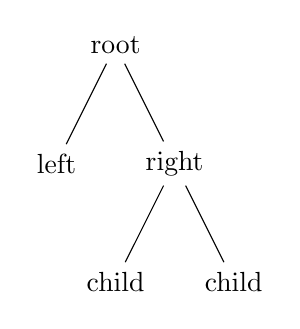
\begin{tikzpicture}
\node {root}
    child {node {left}}
    child {node {right}
    child {node {child}}
    child {node {child}}
    };
\end{tikzpicture}
Allway use \verb|\begin{tikzpicture}| and
\verb|\end{tikzpicture}| to open and close
\end{document}
\end{examplecode}

In order to skip the complications, the verbatim content is classified into
three types:

\begin{description}[font=\sffamily\small, noitemsep,leftmargin=*,style=nextline]
\item[Verbatim standard] These are the classic code writing environments, such
as \texttt{verbatim} and \texttt{verbatim*}.

\item[Verbatim write] They are where you write a file directly on the disk,
such as \texttt{filecontents} or \texttt{VerbatimOut}.

\item[Verbatim inline] Are the commands in which verbatim content is written
in the same line, such as \texttt{$\backslash$verb$\vert$code$\vert$}.
\end{description}

The general process that is carried out when reading the input file is simple
to describe (but difficult to program):

\begin{quotation}
When browsing the file look for the words \lstinline[style=inline]|\begin{| and \lstinline[style=inline]|\end{| in 
verbatim standard, verbatim write, verbatim inline and commented lines, if it finds them, it converts 
them to \lstinline[style=inline]|\BEGIN{| and \lstinline[style=inline]|\END{| (uppercase), then places all the environments 
to extract inside the \lstinline[style=inline]|\begin{preview}|\ldots \lstinline[style=inline]|\end{preview}|, exports them and 
then undoes the changes.
\end{quotation}

As an example:

The vast majority of packages that provide these environments and commands is
supported automatically, otherwise, you can use some of the options of the script.


The script asume a two verbatim environments, a verbatim write content and
verbatim standart content, all material included in these environments is
ignored. Auto detects by default the environments generated by the \pkgname{minted},
\pkgname{listings} and other.

\subsection{Verbatim inline}
\label{sec:verbatim:inline}
The script supports most verbatim inline commands. If your command is not
supported by default or the script can not capture, you can use the option
\cmdopt{myverb}.

The following consideration should be kept in mind for packages that use
abbreviations for verbatim commands, such as \pkgname{shortverb} or
\pkgname{doc} for example.

The script detects the use of the commands \ics{DefineShortVerb}, \ics{lstMakeShortInline}
and \ics{MakeSpecialShortVerb}.

\begin{examplecode}
\DefineShortVerb
\lstMakeShortInline
\MakeSpecialShortVerb
\end{examplecode}

That is, if a package defines it internally, the script will not be able
to process it correctly. The solution is quite simple, just add in input file:

\begin{examplecode}
\UndefineShortVerb
\DefineShortVerb
\end{examplecode}

depending on the package you are using.

\subsection{Verbatim standart}
\label{sec:verbatim:std}
The following list is considered as standard verbatim environments:

\begin{multicols}{4}
\begin{itemize}[font=\sffamily\small, noitemsep,leftmargin=*]
\sffamily\small
\item Example
\item CenterExample
\item SideBySideExample
\item PCenterExample
\item PSideBySideExample
\item verbatim
\item Verbatim
\item BVerbatim
\item LVerbatim
\item SaveVerbatim
\item PSTcode
\item LTXexample
\item tcblisting
\item spverbatim
\item minted
\item listing
\item lstlisting
\item alltt
\item comment
\item chklisting
\item verbatimtab
\item listingcont
\item boxedverbatim
\item demo
\item sourcecode
\item xcomment
\item pygmented
\item pyglist
\item program
\item programl
\item programL
\item programs
\item programf
\item programsc
\item programt
\end{itemize}
\end{multicols}

And capture environments defined in main file from commands:

\begin{multicols}{2}
\begin{itemize}[font=\sffamily\small, noitemsep,leftmargin=*]
\sffamily\small
\item \ics{DefineVerbatimEnvironment}
\item \ics{NewListingEnvironment}
\item \ics{DeclareTCBListing}
\item \ics{ProvideTCBListing}
\item \ics{lstnewenvironment}
\item \ics{newtabverbatim}
\item \ics{specialcomment}
\item \ics{includecomment}
\item \ics{newtcblisting}
\item \ics{NewTCBListing}
\item \ics{newverbatim}
\item \ics{NewProgram}
\end{itemize}
\end{multicols}

If any of the environments is not supported by default or the script can
not capture it, you can use the option \cmdopt{verbenv} to add.

\subsection{Verbatim write}
\label{sec:verbatim:write}
The following list is considered as verbatim write environments:

\begin{multicols}{3}
\begin{itemize}[font=\sffamily\small, noitemsep,leftmargin=*]
\sffamily\small
\item filecontents
\item tcboutputlisting
\item tcbexternal
\item extcolorbox
\item extikzpicture
\item VerbatimOut
\item verbatimwrite
\item filecontentsdef
\item filecontentshere
\end{itemize}
\end{multicols}

And the script tries to capture the defined environments by means of:
\begin{multicols}{2}
\begin{itemize}[font=\sffamily\small, noitemsep,leftmargin=*]
\sffamily\small
\item \ics{renewtcbexternalizetcolorbox}
\item \ics{renewtcbexternalizeenvironment}
\item \ics{newtcbexternalizeenvironment}
\item \ics{newtcbexternalizetcolorbox}
\end{itemize}
\end{multicols}

If any of the environments is not supported by default or the script can't
capture it, you can use the option \cmdopt{writenv} to add.

\section{How it works}
\label{sec:howtowork}
\subsection{Call the script}
The syntax for \myscript{} is simple:

\begin{examplecmd}
[user@machine ~:]§ ltximg `\small \meta[type=tt,cf=red]{compiler} \oarg[type=tt,cf=gray]{options} \marg[type=tt]{file}{.}\marg[type=tt]{ext}`
\end{examplecmd}

The .\marg{ext} valid for input \marg{file} are \fext{tex} or \fext{ltx}.
The \meta[type=tt,cf=red]{compiler} need to pass used \texttt{\small\bfseries\textcolor{optcolor}{-\/-}} 
and \oarg[type=tt,cf=gray]{options} need to pass used \texttt{\small\bfseries\textcolor{optcolor}{-\/-}} 
or \texttt{\small\bfseries\textcolor{optcolor}{-}} in command line. For example:

\begin{examplecmd}
[user@machine ~:]§ ltximg -e -p -j --srcenv --imgdir pics -o test-out test-in.ltx
\end{examplecmd}

produce a file \marg{test-out.ltx} with all environments extracted converted to \ics{includegraphics} and create
\sysdir{pics} dir whit all images format (\iext{pdf}, \iext{eps}, \iext{png}, \iext{jpg})
and source code in separate files using (pdf)LaTeX whit \pkgname{preview} package.

%-output-directory
The script support bundling for short options:

\begin{examplecmd}
[user@machine ~:]§ ltximg -epj --srcenv --imgdir=pics -o test-out  test-in.ltx
\end{examplecmd}

\subsection{Internal process}
\label{sec:internal:proc}
The script works in varius steps for create image files, source code and output file
\emph{without} suported environments.

\begin{description}[font=\sffamily\small, noitemsep,leftmargin=*,style=nextline]
\item[Comment and ignore] The first step is to check the input file and create a
directory \sysdir{images} to save the images and source files of each environment
to extract. At this point the entire input file (\textsf{test.tex}) is read in
memory to be processed as follows:

\begin{enumerate}
\item  Once it is read in memory, it begins to analyze verbatim and verbatim
write environments.

\item  Change problematic inline verbatim from varius package (lstlisting,
LTXexample, Verbatim, comment, alltt, minted, tcblisting, etc) and commented
lines whit \%.
\end{enumerate}

Once this process is completed, you can start with the process of extracting
and converting environments.

\item[Create source file] In this second stage the script will process in
two ways depending on the options included:

\begin{enumerate}
\item If script is call whitout \cmdopt[n]{noprew} option, adds the
following lines to the beginning of the test.tex in memory and save file
test-fig-random.tex in \sysdir{tmp} dir:

\begin{examplecode}
\AtBeginDocument{%
\RequirePackage[active,tightpage]{preview}
\renewcommand\PreviewBbAdjust{-60pt -60pt 60pt 60pt}}%
% rest of input file
\end{examplecode}

\item If script is call whit \cmdopt[n]{noprew} option, all environment code
its put inside the \env{preview} environment. The begin/end lines are only used
as delimiters for extracting the content without using the package \pkgname{preview}.
It should be noted that in this mode all the code that wishes to be converted
must be within the environment or within tags. The generated file test-fig-rand.tex
in \sysdir{tmp} dir has the same preamble, but it only contains the environments that
we want to extract.
\end{enumerate}

\item[Generate files] Now, the \emph{script} run \marg[type=tt,cf=red]{compiler}
whit \prgopt*{recorder} \prgopt*{shell-escape} option over \oarg{test-fig-random.tex},
generate a one pdf file whit all environment, separate in individual files (test-fig-1.tex, test-fig-2.tex, etc)
and copy to \sysdir{images}. The file test-fig-random.tex is moved to the \sysdir{images} dir
with the name test-fig-all.tex.
\end{description}
Once the process is finished \sysdir{tmp} dir and most of temporary files
generated are deleted.

\section{Extract content}
\label{sec:extract}
The environments: 
\begin{multicols}{3}
\begin{itemize}[font=\sffamily\small, noitemsep,leftmargin=*]
\item \env{pspicture}
\item \env{tikzpicture}
\item \env{pgfpicture}
\item \env{psgraph}
\item \env{postscript} 
\item \env{PSTexample} 
\end{itemize}
\end{multicols}
(including a starred \texttt{\small\bfseries\textcolor{red}{*}} version) are suported by default. 
If the environments are nested, the outermost will be extracted.

\subsection{Extract environment}
\label{sec:extract:env}
\DescribeTE{preview}
Environment provide by \pkgname{preview} package. If \env{preview} environments
found in the input file will be extracted and converted these. Internally
converts all environments to extract in \env{preview} environments.
Is better comment this package in preamble unless the option \cmdopt[n]{noprew}{} is
used.

\vspace{\baselineskip}

\DescribeTE{pspicture}
Environment provide by \pkgname{pstricks} package. The plain
syntax \lstinline[style=inline]|\pspicture ... \endpspicture| its converted to
\lstinline[style=inline]|\begin{pspicture} ... \end{pspicture}|.
\vspace{\baselineskip}

\DescribeTE{psgraph}
Environment provide by \pkgname{pst-plot}. The script converts the plain syntax \lstinline[style=inline]|\psgraph ... \endpsgraph|
to latex syntax \lstinline[style=inline]|\begin{psgraph} ... \end{psgraph}|.

\vspace{\baselineskip}

\DescribeTE{postscript}
Environment provide by \pkgname{pst-pdf} and \pkgname{auto-pst-pdf} packages.
Since the \pkgname{pst-pdf} and \pkgname{auto-pst-pdf} packages internally use
the \pkgname{preview} package, is better comment this in preamble.

\vspace{\baselineskip}

\DescribeTE{tikzpicture}
Environment provide by \pkgname{tikz} package. The script convert the plain
syntax \lstinline[style=inline]|\tikzpicture ... \tikzpicture| to latex syntax
\lstinline[style=inline]|\begin{tikzpicture} ... \end{tikzpicture}|
but no a short \lstinline[style=inline]|\tikz|.
\vspace{\baselineskip}

\DescribeTE{pgfpicture}
Environment provide by \pkgname{pgf} package. Since the script uses a
\emph{recursive regular expression} to extract environments, no presents problems
if present \lstinline[style=inline]|pgfinterruptpicture|.
\vspace{\baselineskip}

\DescribeTE{PSTexample}
Environment provide by \pkgname{pst-exa} packages. The script automatically
detects the \lstinline[style=inline]|\begin{PSTexample} ... \end{PSTexample}| environments and
processes them as separately compiled files. The user should have loaded the
package with the [\pkgopt{swpl}] or [\pkgopt{tcb}] option and run the script
using \cmdopt{latex}{} or \cmdopt{xetex}.

\subsection{Extract whit DTXtag}
\label{sec:extract:tag}
\DescribeTE*{ltximg}
All content included between \lstinline[style=inline]|%<*ltximg> ... %</ltximg>| is extracted. 
The tags can not be nested and should be at the beginning of the line and in separate lines.

\begin{examplecode}
% no space before open tag %<* 
%<*ltximg>
code to extract and convert
%</ltximg>
% no space before close tag %</ 
\end{examplecode}

\subsection{No extract and remove}
\label{sec:noextract:tag}
\DescribeTE{nopreview}
Environment provide by \pkgname{preview} package. Internally the script
converts all no extract environments to \lstinline[style=inline]|\begin{nopreview} ... \end{nopreview}|.
Is better comment this package in preamble unless the option \cmdopt[n]{noprew}{} is used.
\vspace{\baselineskip}

\DescribeTE*{noltximg}
All content betwen \lstinline[style=inline]|%<*noltximg> ... %</noltximg>| are ignored and no
extract. The start and closing of the tag must be at the beginning of the line.

\begin{examplecode}
% no space before open tag %<* 
%<*noltximg>
no extract this lines
%</noltximg>
% no space before close tag %</ 
\end{examplecode}
\vspace{\baselineskip}

\DescribeTE*{remove}
All content betwen \lstinline[style=inline]|%<*remove> ... %</remove>| are deleted in the output file. The start and closing
of the tag must be at the beginning of the line.

\begin{examplecode}
% no space before open tag %<* 
%<*remove>
this lines are removed in output file
%</remove>
% no space before close tag %</ 
\end{examplecode}

\newpage
\section{Command line options}
\label{sec:optcmdline}

\DescribeCmd[h]{help}{bolean}{off}
Display a short help text and exit.

\DescribeCmd[l]{license}{bolean}{off}
Display a license text and exit.

\DescribeCmd[v]{version}{bolean}{off}
Display the current version (1.5) and exit.

\DescribeCmd[d]{dpi}{int}{150}
Dots per inch for images files.

\DescribeCmd[t]{tif}{bolean}{off}
Create a .\iext{tif} images files using \prgname{ghostscript}. The line before this options is:

\begin{examplecmd}
§ gs -q -dNOSAFER -sDEVICE=tiff32nc -r 150
\end{examplecmd}

\DescribeCmd[b]{bmp}{bolean}{off}
Create a .\iext{bmp} images files using \prgname{ghostscript}. The line before this options is:

\begin{examplecmd}
§ gs -q -dNOSAFER -sDEVICE=bmp32b -r 150
\end{examplecmd}

\DescribeCmd[j]{jpg}{bolean}{off}
Create a .\iext{jpg} images files using \prgname{ghostscript}. The line before this options is:

\begin{examplecmd}
§ gs -q -dNOSAFER -sDEVICE=jpeg -r 150 -dJPEGQ=100 -dGraphicsAlphaBits=4 \
    -dTextAlphaBits=4
\end{examplecmd}

\DescribeCmd[p]{png}{bolean}{off}
Create a .\iext{png} transparent image files using \prgname{ghostscript}.  The line before this options is:

\begin{examplecmd}
§ gs -q -dNOSAFER -sDEVICE=pngalpha -r 150
\end{examplecmd}

\DescribeCmd[e]{eps}{bolean}{off}
Create a .\iext{eps} image files using \prgname{pdftops}. The line before this options is:

\begin{examplecmd}
§ pdftops -q -eps
\end{examplecmd}

\DescribeCmd[s]{svg}{bolean}{off}
Create a .\iext{svg} image files using \prgname{pdftocairo}. The line before this options is:

\begin{examplecmd}
§ pdftocairo -q -eps
\end{examplecmd}

\DescribeCmd[P]{ppm}{bolean}{off}
Create a .\iext{ppm} image files using \prgname{pdftoppm}. The line before this options is:

\begin{examplecmd}
§ pdftoppm -q -eps
\end{examplecmd}

\DescribeCmd[g]{gray}{bolean}{off}
Create a gray scale for all images using \prgname{ghostscript}. The line before this options is:

\begin{examplecmd}
§ gs -q -dNOSAFER -sDEVICE=pdfwrite -dPDFSETTINGS=/prepress       \
     -sColorConversionStrategy=Gray -dProcessColorModel=/DeviceGray
\end{examplecmd}

\DescribeCmd[f]{force}{bolean}{off}
Try to capture \lstinline[style=inline]|\psset| and \lstinline[style=inline]|\tikzset| to extract

\DescribeCmd[n]{noprew}{bolean}{off}
Create images files whitout preview

\DescribeCmd[m]{margin}{numeric}{0}
Set margins in bp for \scriptname{pdfcrop}.

\DescribeCmd[o]{output}{string}{empty}
Create output file whit all environmets converted in image.  <outname> must not contain extension.

\DescribeCmd{imgdir}{string}{/images}
The folder for save images and source code

\DescribeCmd{verbose}{bolean}{off}
Show verbose information in screen \prgopt*{interaction}

\DescribeCmd{srcenv}{bolean}{off}
Create separate files whit only code environment

\DescribeCmd{srcenv}{bolean}{off}
Create sub files whit preamble and code environment

\DescribeCmd{arara}{bolean}{off}
Use \prgname{arara} for compiler files, need to pass \prgopt*{recorder} option to input file\par
\lstinline[style=inline]|% arara : <compiler> : {options: "-recorder"}|

\DescribeCmd{xetex}{bolean}{off}
Using \prgname*{xelatex} compiler for create images

\DescribeCmd{latex}{bolean}{off}
Using \prgname*{latex}>\prgname*{dvips}>\prgname*{ps2pdf} compiler in input file to create images
and \prgname*{pdflatex} for output file.

\DescribeCmd{dvips}{bolean}{off}
Using \prgname*{latex}>\prgname*{dvips}>\prgname*{ps2pdf} for compiler input and output file

\DescribeCmd{dvipdf}{bolean}{off}
Using \prgname*{latex}>\prgname*{dvipdfmx} process for create images

\DescribeCmd{luatex}{bolean}{off}
Using \prgname*{lualatex} to compiler files

\DescribeCmd{prefix}{string}{fig}
Add prefix append to each file created

\DescribeCmd{norun}{bolean}{off}
Run script, but no create images

\DescribeCmd{nopdf}{bolean}{off}
Don't create a PDF image files

\DescribeCmd{nocrop}{bolean}{off}
Don't run \scriptname{pdfcrop} in image files

\DescribeCmd{myverb}{string}{myverb}
Set verbatim inline command \lstinline[style=inline]|\string|

\DescribeCmd{clean}{doc\textbar pst\textbar tkz\textbar all\textbar off}{doc}
Removes specific text in output file.

\DescribeCmd{extrenv}{list separtate by comma}{empty}
List of other environments to extract, need -- at end\par

\DescribeCmd{skipenv}{list separtate by comma}{empty}

List of environments that should not be extracted and that the script supports
by default, need -- at end.\par

\DescribeCmd{verbenv}{list separtate by comma}{empty}

Add new verbatim environment suport, need -- at end.\par

\DescribeCmd{writenv}{list separtate by comma}{empty}

Add new verbatim write environment support, need -- at end.\par

\DescribeCmd{deltenv}{list separtate by comma}{empty}
Delete environment in output file,  need -- at end.\par

\newpage
\section{Options in input file}
\label{sec:optfile}

Many of the ideas in this section are inspired by the \prgname{arara} program (I adore it).
A very useful way to pass options to the script is to place them in commented
lines at the beginning of the file, very much in the style of \prgname{arara}.

\DescribeOptFile*{\meta[ac=gray,cf=gray]{argument}}{option one, option two, option three, \ldots}
\DescribeOptFile*{\meta[ac=gray,cf=gray]{argument}}{option one, option two, option three, \ldots}[!]

The vast majority of the options can be passed into the input file. These should be put at
the beginning of the file in commented lines. If you are going to create
an output file and you do not want these lines to remain, it is better to
place them inside the \lstinline[style=inline]|%<*remove> ... %</remove>|. Like this:

\begin{examplecode}
%<*remove>
% ltximg : options : {png,srcenv,xetex}
% ltximg : extrenv : {description}
%</remove>
\documentclass{article}
\begin{document}
    some content
\end{document}
\end{examplecode}

\DescribeOptFile{options}{opt1=val, opt2=val, \ldots, bolean}
This line is to pass the types of format you want to create\par

\DescribeOptFile{extrenv}{extract env one, extract env two, \ldots}
This line is to indicate to the script which environments, not supported by
default, are extracted.

\DescribeOptFile{skipenv}{env one,env two, \ldots}
This line is to indicate to the script which environments, of the ones
supported by default, should not be extracted.

\DescribeOptFile{verbenv}{verb one,verb two, \ldots}
This line is to indicate to the script which environments, its considerate a verbatim.

\DescribeOptFile{writenv}{write one,write two,\ldots}
This line is to indicate to the script which environments its consider writeout.

\DescribeOptFile{deltenv}{delete env one, delete env two, \ldots}
This line is to indicate to the script which environments are deleted.
The deletion process only occurs if an output file is defined. It runs after
having extracted and created the images completely and only affects the output
file. For example, if the input file is something like this:
\begin{examplecode}
% ltximg : options : {png,srcenv}
% ltximg : deltenv : {enumerate}
\documentclass[10pt]{article}
\begin{document}
    some content
\end{document}
\end{examplecode}
and the following line is used:
\begin{examplecmd}
[user@machine~:]§ ltximg -o `\small\meta{file-out} \meta{file-in}.\meta{ext}`
\end{examplecmd}
\newpage
%\changes{v1.0}{2016/10/07}{Beta for first public release}
\PrintChanges
\IndexPrologue{\section*{Index} The index entries}
\PrintIndex
\end{document}
